\begin{tikzpicture}[align=center]

    \node[inner sep=0pt] (user) {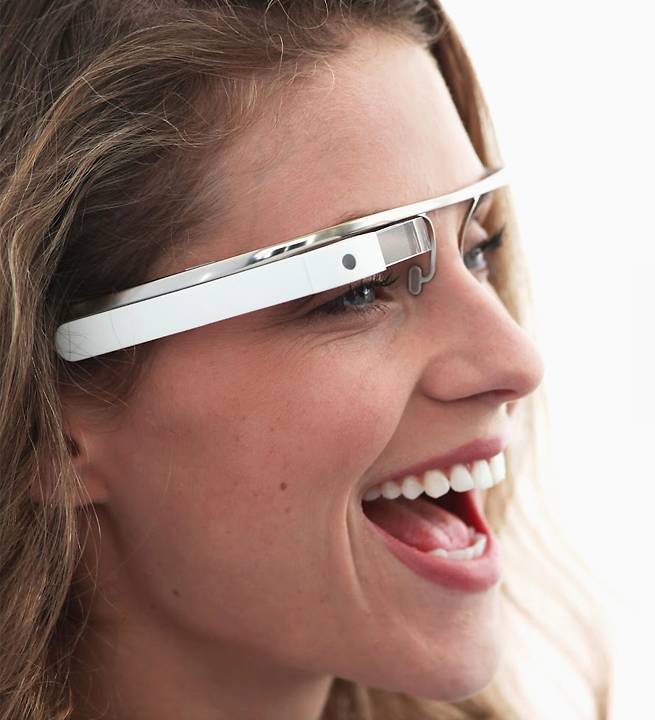
\includegraphics[height=.2\textheight]{img/google-glass.png}};
    \node[inner sep=0pt, right=30mm of user] (arrowsplit) {};

    \matrix [column sep=10mm,row sep=10mm, right=10mm of arrowsplit] (mtx) {
        \node[draw, rectangle, rounded corners=1mm, minimum height=10mm, fill=white!60!orange,
            minimum width=20mm, anchor=center] (record) {Recorder};
        & \node[inner sep=0pt, anchor=center] (trace) {
\includegraphics[height=.12\textheight]{img/floppy.png}}; \\

        \node [inner sep=0pt, anchor=center] (server) {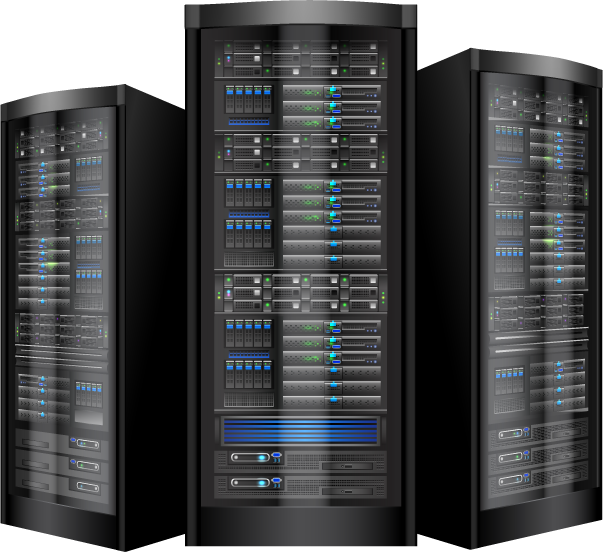
\includegraphics[height=.2\textheight]{img/server.png}}; & \\
    };

    \node[inner sep=0pt, below=5mm of server] (serverarrowanchor) {};

    \draw[very thick, line cap=round] (user) edge[] node[below] (sensorlabel) {Sensory\\Inputs} (arrowsplit.center);

    \draw[very thick, line cap=round, -{Latex[length=2.5mm]}]
    (arrowsplit.center) |- node[] {} (record);

    \draw[very thick, line cap=round, -{Latex[length=2.5mm]}]
    (arrowsplit.center) |- node[] {} (server);

    \draw[thick, line cap=round, -{Latex[length=1.5mm]}]
    (record) -- (trace);

    \draw[very thick, line cap=round]
    (server.south) -- (serverarrowanchor.center);

    \draw[very thick, line cap=round, -{Latex[length=2.5mm]}]
    (serverarrowanchor.center) -| (user.south); 

    \node[inner sep=0pt, anchor=center, below=16mm of sensorlabel] {Feedback};

    %\draw[thick, line cap=round, -{Latex[length=2.5mm]}, shorten >=0pt]
    %(record.east) -- (trace.west);


    %(inputs.north) -- (record.south);

    %\draw[white!30!violet, line width=.5mm, line cap=round]
    %(inputs.160) -- (record.225)
    %(inputs.20) -- (record.315);
\end{tikzpicture}